\newpage
\solutions{Indukcja matematyczna}

\begin{problem}{1} 
	Wykazać, że suma miar kątów w $n$-kącie wypukłym wynosi ${(n - 2) \cdot 180\degree}$.
\end{problem}

\noindent
Zauważmy, że dla $n = 3$ teza jest znanym faktem -- mianowicie suma kątów w trójkącie wynosi $180\degree$.


\begin{center}
	\begin{tikzpicture}[scale=0.6]
		\tkzDefPoint(0,0){A}
		\tkzDefPoint(4,0){B}
		\tkzDefPoint(6,1){C}
		\tkzDefPoint(5,3){D}
		\tkzDefPoint(3,3){E}
		\tkzDefPoint(-1,2){F}
		\tkzDrawSegments(A,B B,C C,D D,E E,F F,A)
		\tkzDrawSegments[dashed](B,D)
		\tkzDrawPoints(A,B,C,D,E,F)
	\end{tikzpicture}
\end{center}

\noindent
Załóżmy, że dla każdego $n$-kąta wypukłego suma jego kątów wynosi ${(n - 2) \cdot 180\degree}$. Rozpatrzmy dowolny $(n+1)$-kąt wypukły. Zauważmy, że ma on więcej niż trzy wierzchołki, więc możemy ,,odciąć'' trójkąt złożony z trzech kolejnych wierzchołków. Podzielimy w ten sposób $(n + 1)$-kąt na $n$-kąt i trójkąt. Korzystając z wypukłości rozpatrywanego wielokąta możemy zauważyć, że suma miar jego kątów wewnętrznych jest sumą miar kątów obu tych wielokątów. Wynosi więc ona
\[
	(n - 2) \cdot 180\degree + 180\degree = (n - 1) \cdot 180\degree,
\]
czego należało dowieść.

\vspace{5px}

\begin{problem}{2}
	 Wykazać, że dla każdej dodatniej liczby całkowitej $n$ zachodzi tożsamość
	\[
		1^2 + 2^2 + 3^2 + ... + n^2 = \frac{n(n + 1)(2n + 1)}{6}.
	\]
\end{problem}

\noindent
Sprawdzamy, że dla $n = 1$ postulowana równość zachodzi.
Załóżmy, że równość
\[
	1^2 + 2^2 + 3^2 + ... + n^2 = \frac{n(n + 1)(2n + 1)}{6}
\]
zachodzi dla pewnej liczby $n$. Chcemy wykazać tezę dla $n + 1$, czyli
\[
	1^2 + 2^2 + 3^2 + ... + n^2 + (n + 1)^2 = \frac{(n + 1)(n + 2)(2n + 3)}{6}.
\]
Zauważmy, że sprowadza się ona do wykazania tożsamości
\[
	\frac{n(n + 1)(2n + 1)}{6} + (n + 1)^2 = \frac{(n + 1)(n + 2)(2n + 3)}{6}.
\]
Przekształcając powyższą równość równoważnie otrzymujemy kolejno
\begin{align*}
	n(n + 1)(2n + 1) + 6(n + 1)^2 &= (n + 1)(n + 2)(2n + 3), \\
	2n^3 + 3n^2 + n + 6(n + 1)^2 &= 2n^3 + 9n^2 + 13n + 6, \\
	6(n + 1)^2 &= 6n^2 + 12n + 6, \\
	(n + 1)^2 &= n^2 + 2n + 1.
\end{align*}

\begin{problem}{3}
Dana jest następująca gra, zwana \textit{wieżami Hanoi}. Na początku ułożono $n$ dysków na jednej igle tak jak na rysunku. W każdym ruchu gracz może przemieścić dysk na inną igłę, przy czym dysk ten nie może zostać położony na dysk o mniejszej średnicy. Wykazać, że gracz jest w stanie przenieść wszystkie dyski na trzecią igłę.

\begin{center}
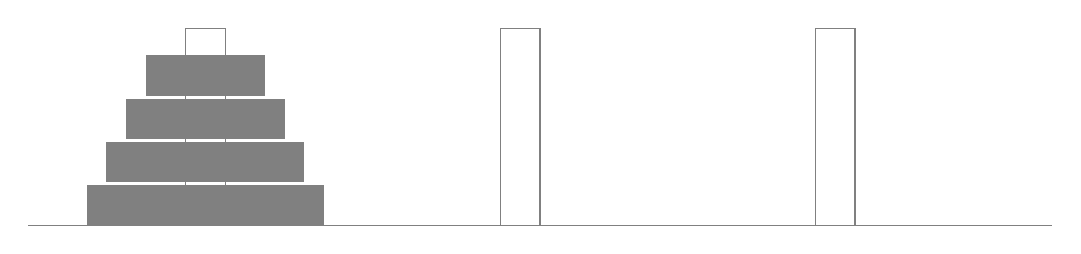
\begin{tikzpicture}[scale=0.5]
	\draw[gray, thin] (0,0) -- (26,0);
	\draw[gray, thin] (4,0) -- (4,5) -- (5,5) -- (5,0);
	\draw[gray, thin] (12,0) -- (12,5) -- (13,5) -- (13,0);
	\draw[gray, thin] (20,0) -- (20,5) -- (21,5) -- (21,0);

	\draw[gray, thin, fill=black!50] (1.5,0) -- (7.5,0) -- (7.5,1) -- (1.5,1) -- cycle;	
	\draw[gray, thin, fill=black!50] (2,1.1) -- (7,1.1) -- (7,2.1) -- (2,2.1) -- cycle;	
	\draw[gray, thin, fill=black!50] (2.5,2.2) -- (6.5,2.2) -- (6.5,3.2) -- (2.5,3.2) -- cycle;	
	\draw[gray, thin, fill=black!50] (3,3.3) -- (6,3.3) -- (6,4.3) -- (3,4.3) -- cycle;
\end{tikzpicture}

\end{center}

\end{problem}

\noindent
Tezę wykażemy indukcją po $n$. Zauważmy, że dla $n = 1$ teza jest oczywista -- wystarczy po prostu przełożyć dysk na trzecią igłę.

\vspace{10px}

\noindent
Załóżmy, że jesteśmy w stanie przełożyć $n - 1$ dysków z pierwszej igły na trzecią. Możemy oczywiście zauważyć, że jest to równoważne chociażby możliwości przełożenia ich z igły pierwszej na drugą.
Przełożenia $n$ dysków dokonujemy w następujący sposób:

\begin{enumerate}
	\item Przekładamy $n - 1$ dysków z góry pierwszej igły na drugą igłę. Zauważmy, że dysk o największym rozmiarze nie przeszkadza nam skorzystać z założenia indukcyjnego, gdyż nie uniemożliwi on wykonania żadnego ruchu.

	\item Dysk pozostawiony na pierwszej igle przekładamy na igłę ostatnią.

	\item Przekładamy $n - 1$ dysków z drugiej igły na trzecią. Analogicznie zauważamy, że obecność jednego dysku na trzeciej igle nie jest problemem.
\end{enumerate}

\begin{problem}{4}
	W przestrzeni danych jest $n \geqslant 3$ punktów, że żadne trzy z nich nie leżą na jednej prostej. Każde dwa z tych punktów połączono odcinkiem o kolorze zielonym lub czerwonym. Wykazać, że można wybrać tak jeden z tych kolorów, aby każde dwa z danych punktów były połączone odcinkiem lub łamaną tego koloru.
\end{problem}

\noindent
Dla $n = 3$ mamy trójkąt. Wybierając kolor, na który pomalowano co najmniej dwa odcinki, postulowana własność będzie spełniona.
\vspace{10px}

\noindent
Załóżmy, że dla teza zachodzi dla $n$ punktów. Rozpatrzmy zbiór $n + 1$ punktów. Wyróżnijmy pewien punkt $P$. Punktów poza $P$ jest dokładnie $n$, więc na mocy założenia istnieje kolor -- bez straty ogólności czerwony -- że pomiędzy każdymi dwoma punktami poza $P$ istnieje łamana tego koloru. 

\begin{minipage}{0.5\textwidth}
\begin{center}
\begin{tikzpicture}
\tkzDefPoint(3,3){P}
\tkzDefPoint(0,2){v_1}
\tkzDefPoint(1.5,0){v_2}
\tkzDefPoint(3,0){v_3}
\tkzDefPoint(5,1){v_4}
\tkzDrawPoints(P, v_1,v_2,v_3,v_4)
\tkzDrawSegments[dashed](v_1,v_2 v_2,v_3 v_3,v_4 v_1,v_4)
\tkzDrawSegments(v_1,v_3 v_2,v_4)
\tkzDrawSegments(P,v_2 P,v_3 P,v_4 v_1,P)
\tkzLabelPoints[above](P)
\end{tikzpicture}\\

\end{center}
\end{minipage}
\begin{minipage}{0.5\textwidth}
\begin{center}
\begin{tikzpicture}
\tkzDefPoint(3,3){P}
\tkzDefPoint(0,2){v_1}
\tkzDefPoint(1.5,0){v_2}
\tkzDefPoint(3,0){v_3}
\tkzDefPoint(5,1){v_4}
\tkzDrawPoints(P, v_1,v_2,v_3,v_4)
\tkzDrawSegments[dashed](v_1,v_2 v_2,v_3 v_3,v_4 v_1,v_4 P,v_4)
\tkzDrawSegments(v_1,v_3 v_2,v_4)
\tkzDrawSegments(P,v_2 P,v_3  v_1,P)
\tkzLabelPoints[above](P)
\end{tikzpicture}\\
\end{center}
\end{minipage}
\begin{center}
Na rysunku zamiast kolorów użyto podziału na linię ciągłą i przerywaną.
\end{center}

Rozpatrzmy dwa przypadki:
\begin{enumerate}
	\item Punkt $P$ jest połączony czerwoną krawędzią z pewnym innym punktem $Q$. Wówczas, wybierając dowolny punkt $X$, na mocy założenia wiemy, że istnieje czerwona ścieżka między $X$ i $Q$. Dokładając do niej odcinek między $P$ i $Q$ otrzymujemy ścieżkę między $P$ oraz $X$.
	Wykazaliśmy, że istnieje ścieżka między punktem $P$ i każdym innym punktem. Łącząc to z faktem, że na mocy założenia indukcyjnego taka ścieżka istnieje między każdą inną parą punktów, otrzymujemy, że dla koloru czerwonego teza jest spełniona.
	\item Punkt $P$ jest połączony z każdym innym punktem zielonym odcinkiem. Wówczas łatwo zauważyć, że pomiędzy każdą parą punktów możemy przejść jednym albo dwoma niebieskimi odcinkami przechodzącymi przez punkt $P$.
\end{enumerate}

\begin{problem}{5}
Dany jest ciąg liczb rzeczywistych
\[
	a_0 \neq 0, 1,\quad a_1 = 1 - a_0,\quad a_{n + 1} = 1 - a_n(1 - a_n). 
\]
Wykazać, że dla wszystkich $n$ 
\[
	a_0a_1a_2...a_n\left(\frac{1}{a_0} + \frac{1}{a_1} + \frac{1}{a_2} + ... + \frac{1}{a_n}\right) = 1.
\]
\end{problem}

\noindent
Na początku wykażemy indukcyjnie, że dla każdego $n$ zachodzi równość
\[
	a_{n + 1} = 1 - a_0a_1a_2\cdot ... \cdot a_{n}.
\]
Równość dla $n = 0$ zachodzi na mocy założeń.
Załóżmy, że
\[
	a_{n} = 1 - a_0a_1a_2\cdot ... \cdot a_{n - 1}.
\]
Skoro $a_{n + 1} = 1 - a_n(1 - a_n)$, to otrzymujemy
\[
	a_{n + 1} = 1 - a_n(1 - a_n) = 1 - a_n \cdot a_0a_1a_2\cdot ... \cdot a_{n - 1} = 1 - a_0a_1a_2\cdot ... \cdot a_{n}.
\]
Więc na mocy zasady indukcji matematycznej postulowana równość zachodzi.
\vspace{10px}

\noindent
Teraz przejdziemy do udowodnienia tezy.
Dla $n = 0$ jest ona oczywista.
Załóżmy, że zachodzi równość
\[
	a_0a_1a_2...a_n\left(\frac{1}{a_0} + \frac{1}{a_1} + \frac{1}{a_2} + ... + \frac{1}{a_n}\right) = 1.
\]
Chcemy wykazać, że
\[
	a_0a_1a_2...a_na_{n+1}\left(\frac{1}{a_0} + \frac{1}{a_1} + \frac{1}{a_2} + ... + \frac{1}{a_n} + \frac{1}{a_{n + 1}}\right) = 1.
\]
Przekształcamy powyższą równość korzystając z założenia
\begin{multline*}
	a_0a_1a_2...a_na_{n+1}\left(\frac{1}{a_0} + \frac{1}{a_1} + \frac{1}{a_2} + \frac{1}{a_3} + ... + \frac{1}{a_n} + \frac{1}{a_{n + 1}}\right) = \\ = a_{n+1} \cdot a_0a_1a_2...a_n\left(\frac{1}{a_0} + \frac{1}{a_1} + \frac{1}{a_2} + ... + \frac{1}{a_n}\right) + a_0a_1a_2...a_n = \\ = a_{n + 1} + a_0a_1a_2...a_n = 1 - a_0a_1a_2...a_n + a_0a_1a_2...a_n = 1.
\end{multline*}

\begin{problem}{6}
	Wykazać, że planszę o wymiarach $2^n \times 2^n$ dla pewnego $n \geqslant 1$ z usuniętym jednym z rogów da się przykryć pewną liczbą $L$ klocków(takich jak na rysunku). Klocki można obracać.

	\begin{center}
		\begin{tikzpicture}[scale=0.5]
	    \tkzDefPoint(0,0){v_1}
	    \tkzDefPoint(2,0){v_2}
	    \tkzDefPoint(2,2){v_3}
	    \tkzDefPoint(1,2){v_4}
	    \tkzDefPoint(1,1){v_5}
	    \tkzDefPoint(0,1){v_6}
	    \tkzDefPoint(1,0){A}
	    \tkzDefPoint(2,1){B}

	    \tkzDrawSegments(v_1,v_2 v_2,v_3 v_3,v_4 v_4,v_5 v_5,v_6  v_6,v_1)
	    \tkzDrawSegments(v_5,A)
	    \tkzDrawSegments(v_5,B)
		\end{tikzpicture}
	\end{center}
\end{problem}

\noindent
Zauważmy, że plansza $2\times2$ z usuniętym rogiem jest w istocie L-klockiem, więc da się ją pokryć.

\begin{center}
	\begin{tikzpicture}[scale=0.3]
    \tkzDefPoint(0,0){A}
    \tkzDefPoint(0,10){B}
    \tkzDefPoint(10,10){C}
    \tkzDefPoint(10,0){D}
    \tkzDefPoint(9,0){P1}
    \tkzDefPoint(9,1){P2}
    \tkzDefPoint(10,1){P3}
    \tkzDrawSegments(A,B B,C C,D D,A)
    \tkzDrawSegments(P2,P1 P3,P2)


    \tkzDefPoint(5,0){G1}
    \tkzDefPoint(5,10){G2}
    \tkzDefPoint(0,5){G3}
    \tkzDefPoint(10,5){G4}
    \tkzDrawSegments(G1,G2 G3,G4)

    \tkzDefPoint(4,4){T1}
    \tkzDefPoint(4,6){T2}
    \tkzDefPoint(6,6){T3}
    \tkzDefPoint(6,5){T4}
    \tkzDefPoint(5,4){T5}
    \tkzDrawSegments(T1,T2 T2,T3 T3,T4 T1,T5) 
	\end{tikzpicture}\\
\end{center}

\noindent
Załóżmy, że dla planszy $2^{n - 1} \times 2^{n - 1}$ istnieje szukane pokrycie. Pokrycie dla planszy $2^{n} \times 2^{n}$ konstruujemy następująco. Dzielimy planszę dwiema prostymi na trzy jednakowe części i czwartą taką samą, tylko bez rogu. Kładziemy jeden klocek na środku, tak jak na rysunku. Wówczas plansza jest podzielona na cztery jednakowe puste części, które na mocy założenia indukcyjnego można pokryć.

\begin{problem}{7}
Niech $n$ będzie nieparzystą liczbą naturalną, a liczby $x_1,\; x_2,\; ...,\; x_n$ będa parami różne. Dla każdych dwóch liczb $x_i$ oraz $x_j$ zapisano na tablicy wartość bezwzględną ich różnicy. Wykazać, że można podzielić zapisane liczby na dwa zbiory o równej sumie.
\end{problem}
\noindent
Przez multizbiór rozumiemy zbiór w którym jeden element może występować kilka razy.
Załóżmy, że $x_1 \geqslant x_2 \geqslant ... \geqslant x_n$. 
\vspace{10px}

\noindent
Wykażemy tezę dla $n = 3$. Podział na zbiory $\{x_1 - x_2, x_2 - x_3\}$ oraz $\{x_1 - x_3\}$ spełnia warunki zadania.
\vspace{10px}

\noindent
Załóżmy, że teza zachodzi dla $2n + 1$, wykażemy ją dla $2n + 3$.
Rozpatrzmy szukany podział multizbioru różnic zbioru $\{x_1, x_2, ..., x_{2n + 1}\}$ na multizbiory $A$ i $B$ o równej sumie elementów.
Dorzucamy do multizbioru $A$ liczby
\[
	{x_{2k+3}-x_{2k+1}, \; x_{2k+3}-x_{2k},\; \cdots, \; x_{2k+3}-x_{k+2}} \quad \text{i} \quad {x_{2k+2}-x_{k+1},\; \cdots, \; x_{2k+2}-x_1},
\]
a do multizbioru $B$ liczby
\begin{gather*}
	x_{2k+3} - x_{2k+2} \quad \text{i} \quad x_{2k+2} - x_{2k+1},\; x_{2k+2} - x_{2k},\; \cdots,\; x_{2k+2} - x_{k}  \\ \text{oraz} \quad {x_{2k+3} - x_{k-1},\; \cdots, \; x_{2k+3}-x_1}.
\end{gather*}
Łatwo sprawdzić, że suma dorzuconych elementów jest równa. Stąd wynika, że otrzymane zbiory również mają równą sumę elementów, co jest równoważne tezie.